\chapter{Concept and Design}
\label{cha:conceptanddesign}

\section{General}

\section{Requirements and Challenges}

\subsection{Requirements}

\subsubsection{GDPR compliance}
The General Data Protection Regulation (GDPR) is a regulation by the European Parliament, Council of the European Union and the European Commission focussed on strengthening EU citizens digital privacy.  Its main focus is on giving citizens control over their digital personal information and simplyfying the regulatory environment for multinational corporations. However it also adds a strict data compliance regime, by penalizing transgressions with up to 4\% worldwide turnover. Furthermore this regulation does not have to be verified by each EU's regulatory body, since it is a EU regulation, compared to an EU directive which has to be ratified by each EU signatory state.

\section{Challanges}
\label{sec:challanges}

\subsection{Security Goals}
\label{sec:securityGoals}

Designing a identity management systems comes with various legal implications. We are referring here to § 9 “Technical and organizational actions” in the “Federal Data Protection Act”\footnote{Translated from the German language “Bundesdatenschutzgesetz”} were an identity management system shell enforce all necessary measures to protect identity information.\cite{bdsg}

So we will focus on the following security goals:
\begin{enumerate}
\item \textbf{Confidentiality:} Data shell be secured on its transmission. This includes the blockchain and communication over the internet. 
\item \textbf{Integrity:} The integrity of the data needs to be assured so that no entity can change identity information without knowledge. 
\item \textbf{Authenticity:} Identity information are protected against unauthorized access. 
\item \textbf{Non-Repudiation:} No entity can deny having taken an action.
\item \textbf{Privacy:} The privacy of a user is preserved while interacting with the system. 
\end{enumerate}

We further also see the blockchain as a world open readable ledger were everyone can read transactions or information stored on the blockchain. So interactions with the blockchain need to ensure to not expose any identity information. 
It is not allowed to store hashes or encryption of claim in the blockchain, since it is a tamper-proof data storage, information can not be removed once written. So if the hash or encryption gets broken the identity information is leaked and can not be removed.  

\section{Processes}

\subsection{Registration}
In order to be part of our distributed digital identity system that we envisioned, it is necessary to register with it first. The registration process consists of the following steps (See Figure \ref{fig:registration_concept}):

\begin{enumerate}
\item \label{registrar_item_one}
The user creates an ethereum address and a private public key pair, the combination of these two are now used as the users digital identity. Jointly they can be used as a digital identity card. They are safely and securely stored in the users own database.
\item \label{registrar_item_two}
For verification and auditing purposes these have to be verified by a trusted party, so that third parties can be sure of the identity of the individuals. We are using a specially designed smart contract, where the user inputs his ethereum address and his public key. Once filled, he writes it to the blockchain and waits for the trusted party, in our case a governmental agency, to check the contents, fulfill and sign the contract.
\item \label{registrar_item_three}
The user now verifies himself using the eID online verification system. After successfully verifiying he sends the governmental agency, entrusted with handling digital identity services, his ethereum address and public key. These are used for the upcoming smart contract verification.
\begin{comment}
DONT NEED: The user can now have his ethereum address and private public key pair verified by a governmental agency.
\end{comment}
\item \label{registrar_item_four}
The aforementioned governmental agency can now check the blockchain for the requesting users registrar contract, verify its content against already received (See \ref{registrar_item_three}) or saved information and then link the existing user to the ethereum address and public key. After extending the database entry the agency now collects all existing claims for that individual, packages them into a single claims object and sends it to the user for his record keeping and claim query construction.  
\item \label{registrar_item_five}
Lastly the agency signs and approves this registrar contract. By adding its signature the user is now a fully registered member within our community. Henceforth he can use this identity to request services and offer claims to and from other registered parties. 
\end{enumerate}

\begin{figure}[ht]
\centering
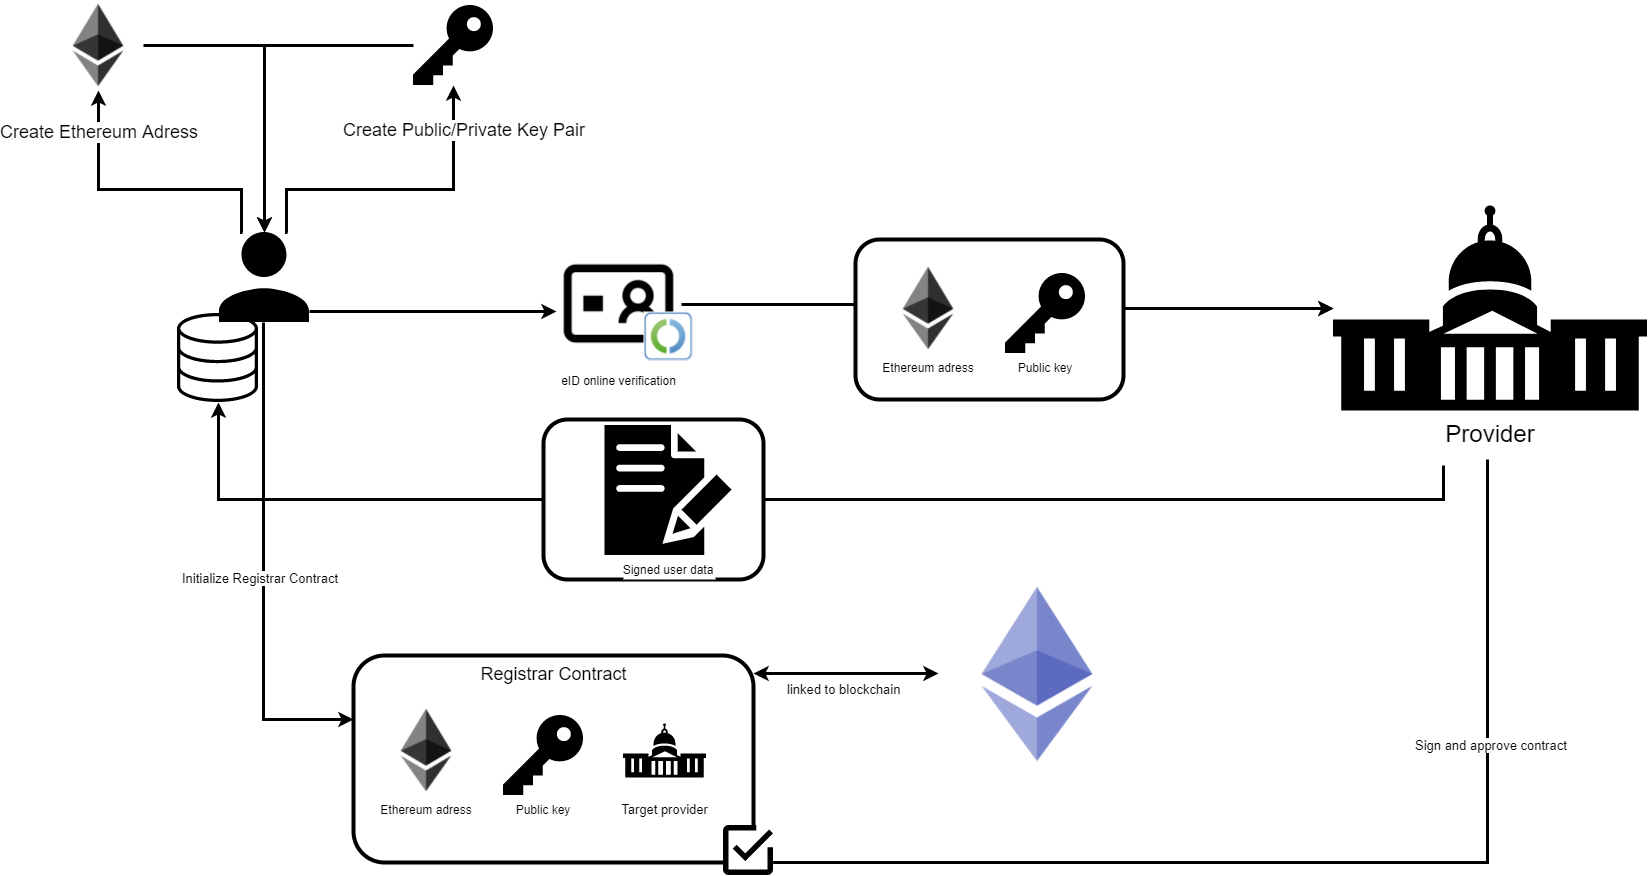
\includegraphics[width=\textwidth]{concept/registration.png}
\caption{Registration}
\label{fig:registration_concept}
\end{figure}

\subsection{Permission Request}
After registration the user is now able to use \projectName{} for identification and verification purposes. Lets consider opening a new bank account using \projectName() for verification.

% Please agument why the user if he is holding signed claims is not providing his claims directly to the requesting provider
% Include the following arguments:
% 1. request shell be populated through the blockchain so that every entity can acknowledge the claim sharing
% 2. populatring thre reuqest through the blockchain gives us the possibility to explicit approve the sharing
% 3. generating a signed query can also have additional attributes like a reuse flag to indicate if the query could be used again if the claim changed
% 4. user don't have to pay for the creation of the smart contract. only for the updating of the signed values

\begin{enumerate}
\item \label{permission_request_item_one}
We have a user called Tom who has just recently moved and is interested in opening a new bank account for his local dealings. He therefore visits a local branch of Bank X and requests a new bank account. He now hands his ethereum address, public key, Name, Address etc. to the bank teller.
\item \label{permission_request_item_two}
The bank teller now enters that information into a \textbf{Request Permission} form and sends it to the government for verification purposes.
\item \label{permission_request_item_three}
The government now writes a new permission request contract into the ethereum blockchain. This contract contains the following information:
\begin{itemize}
\item @EthereumAddress; This is Toms Address, as his information is requested
\item ThirdPartyName; This is the requesting Party's Name Bank 
\item AttributesRequested[GivenName, FamilyName, StreetName, StreetNumber, PostalCode, DateOfBirth, ...]; This is an Array containing all Variables requested by the Third Party
\end{itemize}
\item \label{permission_request_item_four}
The user now polls the blockchain for new messages and finds this permission request by the third party.
\item \label{permission_request_item_five}
Tom now checks each requested attribute and selects the attributes he wants to share with the third party. After his selection a specific query is created imitating his choices.
\end{enumerate}

\begin{figure}[ht]
\centering
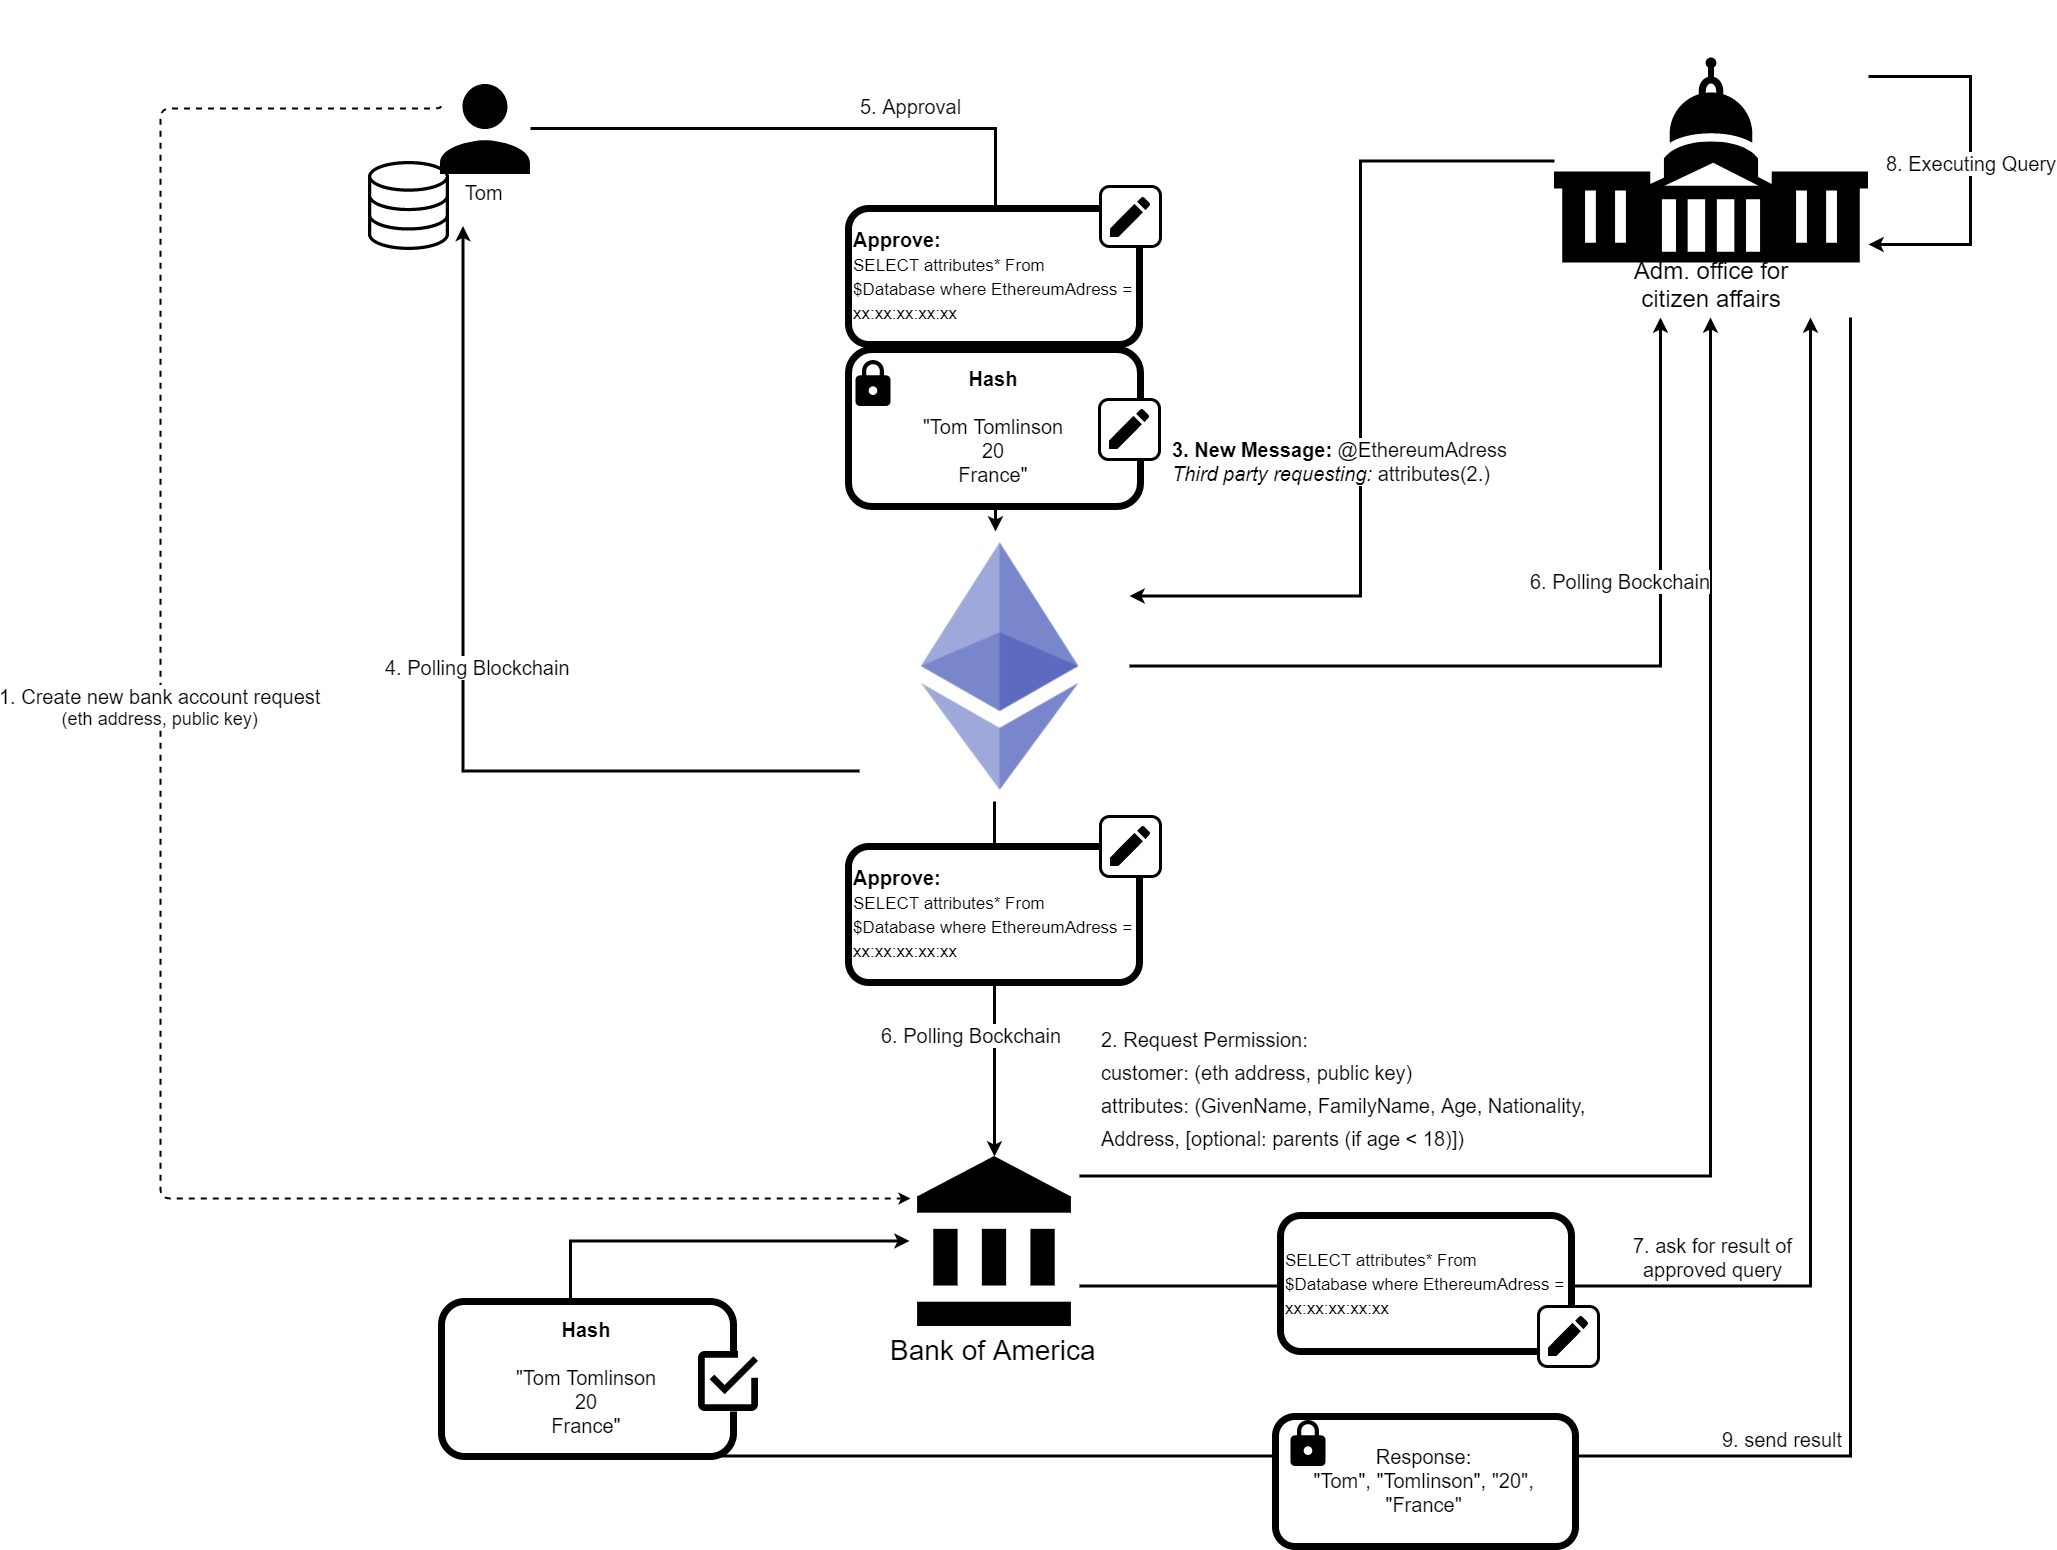
\includegraphics[width=\textwidth]{concept/permission_request_bank.png}
\caption{Permission Request}
\label{fig:permission_request}
\end{figure}

\subsection{Closures}
%Create closure figure in draw.io and insert here
\begin{comment}
\begin{figure}[ht]
\centering
\includegraphics[width=\textwidth]{concept/closure.png}
\caption{Closure}
\label{fig:closure}
\end{figure}
\end{comment}

\subsection{Changing Claims}

\begin{figure}
 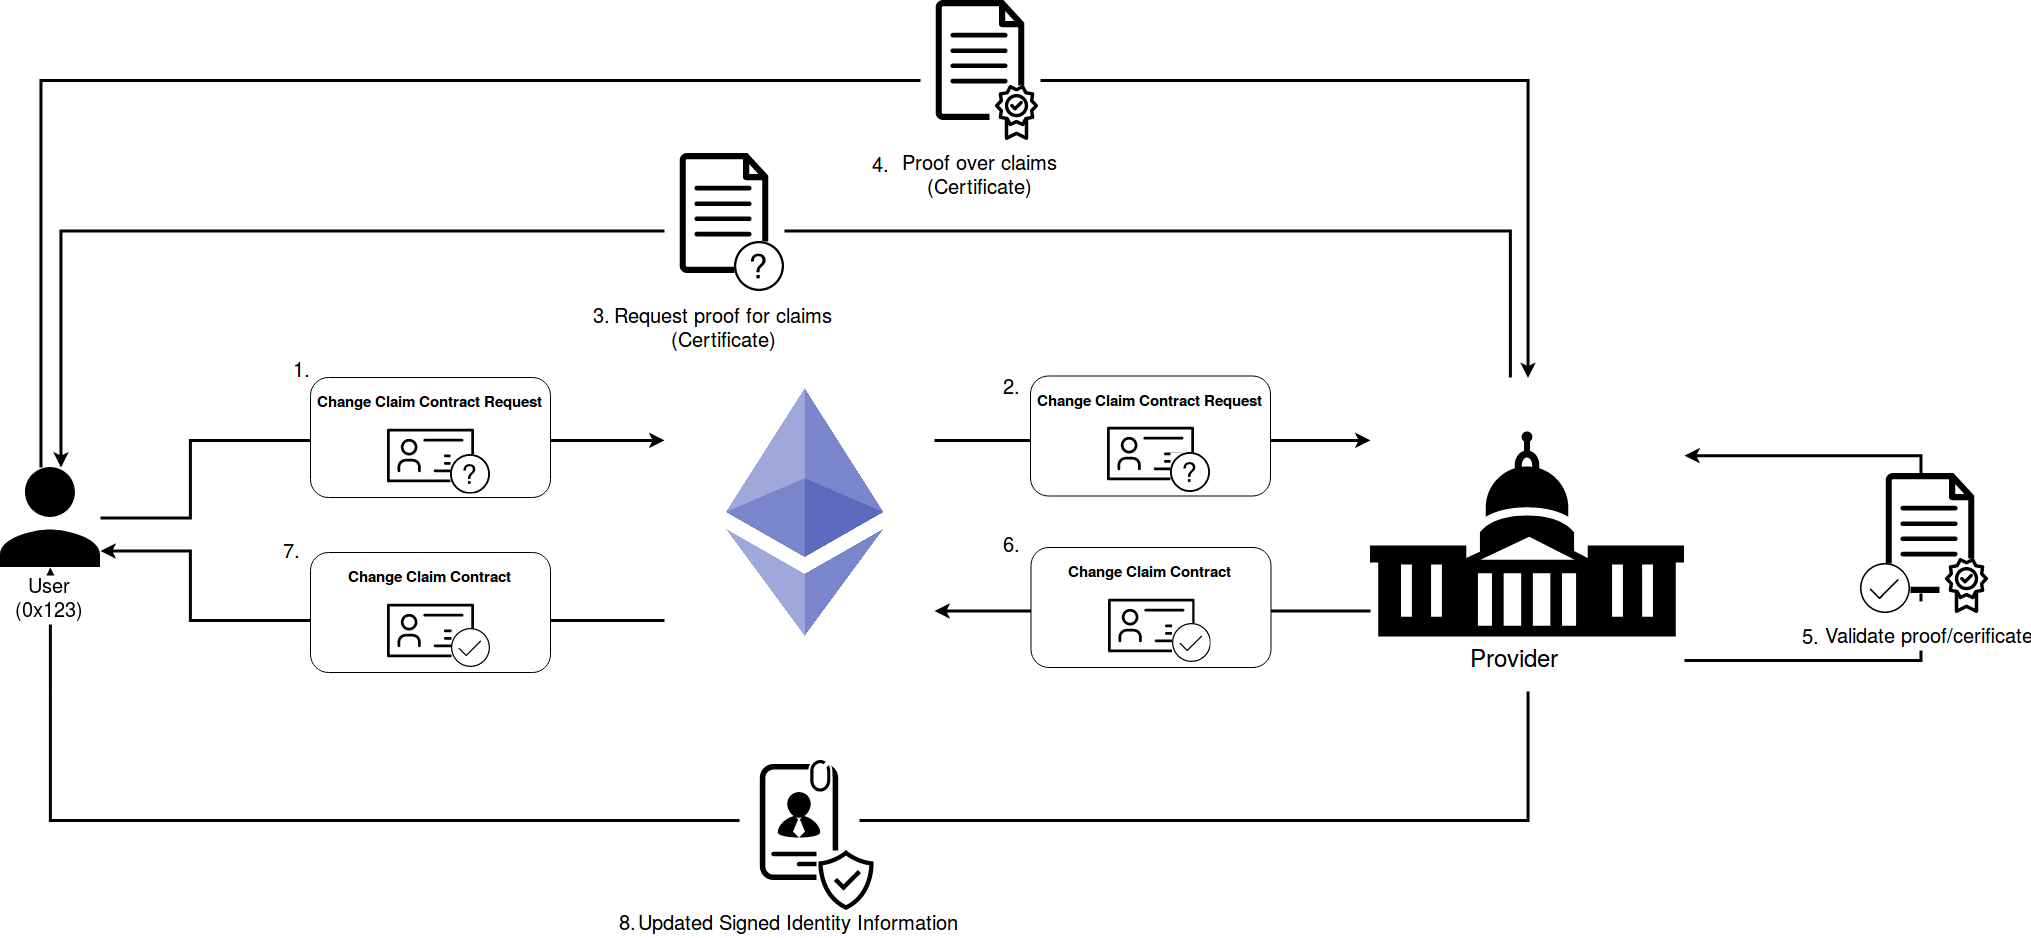
\includegraphics[width=\textwidth]{concept/change_claim.png}
 \centering
\caption{Concept of the change claim workflow. Change claim events are populated trough the blockchain so that every provider holding the same claim for the referenced user can start a new permission request to update the claim values.}
\label{fig:changeClaimsFig}
\end{figure}

Changing claims in a self-sovereign manner with still providing the high level of trust in this claims is a challenge. We evaluated two entry points for this contract: a) the user starts the procedure by sending a “change claim contract request” or b) the government enforces new claims by populating a “change claim contract”. 

For a) the use case is described in section \ref{sec:changeClaimUseCase} where the user may want to change his family name because he got married recently. In the case of b) the government triggers a change claim as an law enforcement (e.g. the user looses his driving license for a certain time) or an other federal institution wants to update the users claims. Each scenarios are described in detail in this section. 

To still serve as a self-sovereign system the user gets the possibility to create a “change claim contract request” (step 1., figure \ref{fig:changeClaimsFig}). This contract itself does not enforce any change of any attributes, but serves as a change claim application. The user states the claim IDs he wants to change in the contract. He may even add additional attributes like a time period to define for how long the claim shell be changed. It is also possible to propose new claims the user want to add by himself. However, this claims needs to be verifiable from the government. The “change claim contract request” is likely addressed at the institution that would have to highest trust level in the system, since the signature over this claims is only trusted as much as the institution itself. In our scenario the government satisfies this trust level. Some might argue that it is not necessary to populate the “change claim contract request” trough the blockchain (since each transaction cost money), but it helps to establish more transparency in our system and relocates power to the user. He decides which claims he wants to change and which new claims he wants to have added to his digital identity. 

The government pulls down the “change claim contract request” and evaluates it in step 2. for which claims it needs a verification, e.g. a certificate. Off-blockchain the user is asked for a proof or certificate over his proposed claims (step 3.). Each provider can define which kind of proof the user must provide to get his claim changed. The level of trust in a provider grows with amount of accuracy the provider puts in his claim validation. The user provides the proof in step 4. Since different provider may accept different proofs, it can be various documents, like photos of his ID card, certificates of his club membership or even audio recordings. However, if the user is not able to provide the necessary proofs contract will be killed and so the change claim request rejected.
The provider validates if the provided proofs satisfies his acceptance criteria in step 5.  If the proofs are sufficient the provider accepts the “Change claim contract request” by setting a flag in the contract, or even removing some claims from the contract were the verification failed (step 6.). 

Now every other provider in the system holding old claim values for the referenced user can create a new permission request to discover the new changed claims from the provider handling the change claim contract. The user still needs to approve the new incoming permission requests. In step 7. the user gets the notification about the successful approval of the change claim contract and queries the provider to retrieve a signed version of his updated claims (step 8.). 

Here the change claim process is finished. However, as mentioned previous there is also a scenario where a federal institution wants to enforce a claim change (for example the temporary removal of driving license). In that case we would directly start at step 6. where the government will publish an already approved “change claim contract” referring to the changed claim IDs and additional values restricting for example the duration of this enforcement. Extern observer of the blockchain will notice that it is an enforced claim change since the user did not provider a “change claim contract request”. In the same was as described previous the provider will take note about the claim change and can setup a new permission request to discover the new claims. As a side note if the user rejects the permission requests the providers holding outdated claim values can simply distrust this values and can decide if they are willing to still provide the user service with outdated values. Please referrer to section \ref{sec:changeClaimUseCase} for a use case.

\subsection{Evaluation}

 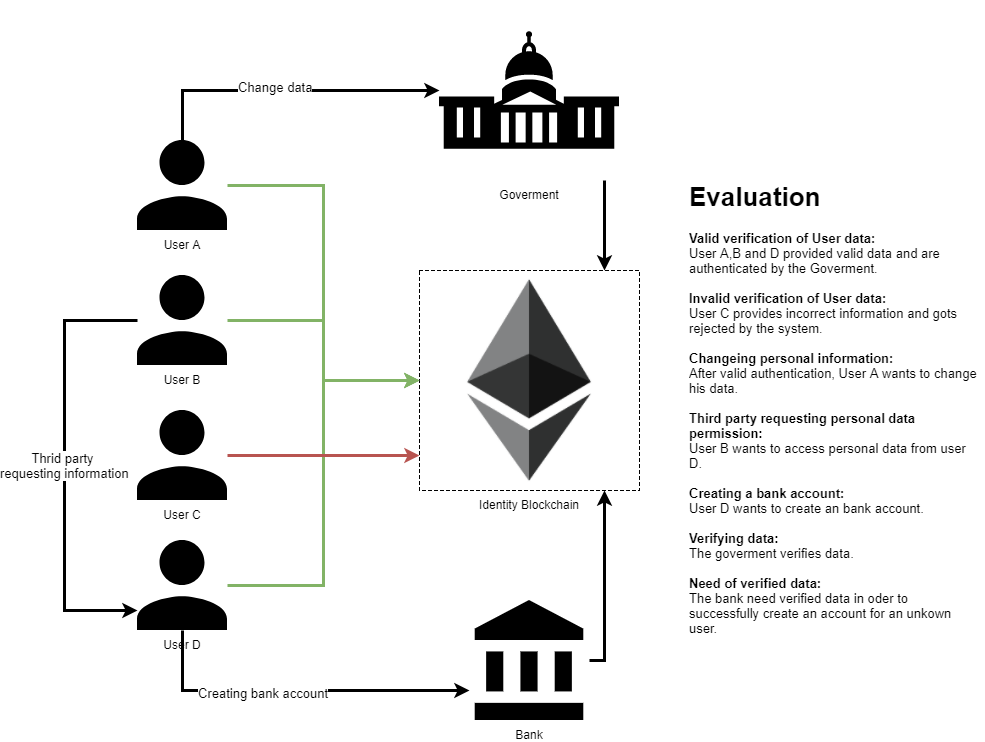
\includegraphics[width=\textwidth]{concept/evaluation.png}
 
\section{Use cases}

\subsection{Change a claim}
\label{sec:changeClaimUseCase}
\textbf{a) User changes claims:}
Lets have a user Bob Bobsen who has recently married Alice Alicson. Since Bob wants to change his family name to Bob Alicon this information needs to be updated in our system. To do so he creates a new “Change Claim Contract Request” holding the “FAMILY\_NAME” claim ID and addressing this contract to the government. The government will ask Bob for his marriage certificate. Bob sends his certificate over a secured connection back. The government, on the other hand, can now verify the new claim by checking Bob's marriage contract. If the certificate is authentic the identity provider publishes an approve transaction to the change claim contract to notify all third parties and other identity providers about the new claim of Bob's digital identity and updates permanently its database. 
Bob does then pull the blockchain, and requests the signed version of his new family name from the government, which he saves in his local database.

\textbf{b) Enforced claim changes:}
Bob has lost his driving license by a moderate traffic crime. Since bob is still holding a signed version of his driving license in his local database he could easy rend a new car. So the government enforces a claim change by publishing a “Change Claim Contract” to the blockchain referencing Bobs ethereum ID, the driving license claim ID and a time period (6 month). Each entity observing the blockchain can within his 6 month distrust the driving license claim value provided by Bob if the provided signature is older then the creation time of the “Change Claim Contract”. However, Bob can query the government for the updated claim values and retrieve the temporary restricted driving license, which is then also trusted, because it is up to date. After 6 month no new claim change contract needs to be setup because an entity can simply compute that the restriction time is expired and that no new claim change was published by the government. 
